\chapter{Hybrid Eulerian-Lagrangian Vortex Particle Method}
\label{ch:hybrid}
%\label{ch:LiteratureReview}

%\section{Eulerian-Lagrangian coupling algorithm}
%The hybrid coupling strategy that we used is a modification of the algorithms developed by Stock \cite{} and Daeninck \cite{}. The coupling scheme is simpler than the Schwarz alternating method, as it required no iteration for the coupling procedure. 
%\section{Theory of Domain Decomposition Method}
% Comparison of hybrid vortex methods.
% choice of hybrid method. Example domain decomposion, coupling technique
%\subsection{Advantage of domain decomposition}
%% What is the advantage?
%% What is the drawback?

Chapter \ref{ch:introduction} introduced the \printAcron{Hybrid Eulerian-Lagrangian Vortex Particle Method}{HELVPM}, a domain decomposition method, where the Eulerian method and the Lagrangian method are used to solve different domains of the fluid.  The algorithm that we use to couple the Lagrangian solver and the Eulerian solver is a modification of the procedures used by Stock and Daeninck. The algorithm is summarized as follows:

	\begin{enumerate}
	\item \textbf{Correct Lagrangian:} Use the solution of the Eulerian domain $\Omega_E$ (in the near-wall region) to correct the solution of the Lagrangian domain $\Omega_L$, that is overlapping the Eulerian domain.
	
	\item \textbf{Evolve Lagrangian:} With the modified solution, evolve the Lagrangian solution from time step $t_n$ to next time step $t_{n+1}$. Chapter \ref{ch:lagrangian} summarizes the procedures of evolving the Lagrangian solution.
	
	\item \textbf{Determine Eulerian boundary conditions:} Use the Lagrangian solution of time $t_{n+1}$ to determine the boundary conditions of the Eulerian domain at $t_{n+1}$.
	
	\item \textbf{Evolve Eulerian:} With the boundary condition, evolve the Eulerian solution from $t_n$ to $t_{n+1}$. Chapter \ref{ch:eulerian} summarizes the procedures of evolving the Eulerian solution.
	\end{enumerate}

We dedicated the chapter \ref{ch:lagrangian} to give an overview on the implementation of the Lagrangian solver. The Lagrangian domain consists of vortex panels that represents the wall-bounded vorticity, and vortex blobs that represents the vorticity everywhere else in the fluid. Chapter \ref{ch:eulerian} was dedicated to introduce the implementation of the Eulerian solver. We decided to use a Finite Element solver that models an incompressible laminar flow using velocity-pressure $\mathbf{u}-p$ formulation. The domain of the Eulerian method is bounded to the body and is used to simulate the vorticity generation from no-slip boundary.

In this chapter, we will elaborate on the coupling of the Eulerian solver and the Lagrangian solver (steps 2 \& 4) to construct the Hybrid Eulerian-Lagrangian Vortex Particle Method. 

\section{Decomposition of the domain}
The hybrid scheme consists  of the decomposition the domain into two subdomains. Figure \ref{fig:hybrid_domains} shows the segregation of the fluid to the near-wall region $\Omega_E$, where an Eulerian solver is used to resolve the near-body region, and a Lagrangian solver is used to resolve the wake region $\Omega_L$.
	\begin{figure}[b]
	\centering
	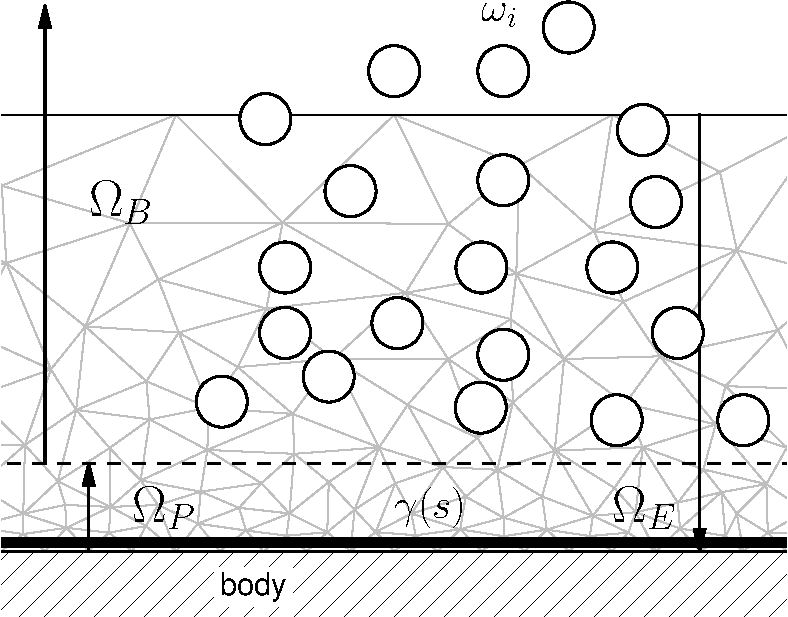
\includegraphics[width=0.45\linewidth]{./figures/hybrid/interpolation/hybrid_domains-crop.pdf}
	\caption{Schematic of the hybrid domain with the Lagrangian domain $\Omega_L: \Omega_P \cup \Omega_B$ and the Eulerian domain $\Omega_E$ resolving the near-wall region $\Omega_E: \Omega_E \subset \Omega_L$.}
	\label{fig:hybrid_domains}
	\end{figure}

The Lagrangian domain $\Omega_L$ is divided into two subdomain: the domain $\Omega_B$ of the vortex blob $\omega(\mathbf{x},t): \mathbf{x} \in \Omega_B$; and the domain $\Omega_P$ of the wall-bounded vortex panel $\gamma(\mathbf{\hat{s}}) \in \Omega_{P}$, the vortex panel domain. In section \ref{sec:boundaryConditions}, we saw that in order to deal the singular wall-bounded vortex sheet distribution, we require a kernels that can represent such distribution. Therefore, the decomposition of the domain is as follows:

	\begin{equation}
	\textit{fluid}:\quad\begin{cases}
	\Omega_E, &\qquad \text{(\textit{Eulerian domain})}  \\
	\Omega_L: \Omega_{P} \cup \Omega_B, &\qquad \text{(\textit{Lagrangian domain})}
	  \end{cases}
	\end{equation}

with the requirements on the domains that:
	\begin{itemize}
	\item Eulerian domain resolves the near-wall region of the Lagrangian domain, $\Omega_E \subset \Omega_L$,
	\item Vortex panel domain is bounded to the wall boundary of the Eulerian domain, $\Omega_P \subset \Omega_E$
	\item Vortex blob domain does not overlap with the vortex panel domain, $\Omega_B \cap \Omega_P : \varnothing$
	\end{itemize}

During the decomposition of the domain, we defined three boundaries, figure \ref{fig:hybrid_config}:
\begin{itemize}
\item No-slip wall boundary of the Eulerian and the vortex panel domain, $\partial \Omega_{\mathrm{wall}}$
\item External boundary of the Eulerian domain where we will prescribe the Dirichlet velocity boundary condition, $\partial \Omega_{E}$.
\item The boundary of the vortex panel domain $\Omega_P$ and the vortex blob domain $\Omega_B$, $\partial \Omega_P$.
\end{itemize}	

	\begin{figure}[t]
	\centering
	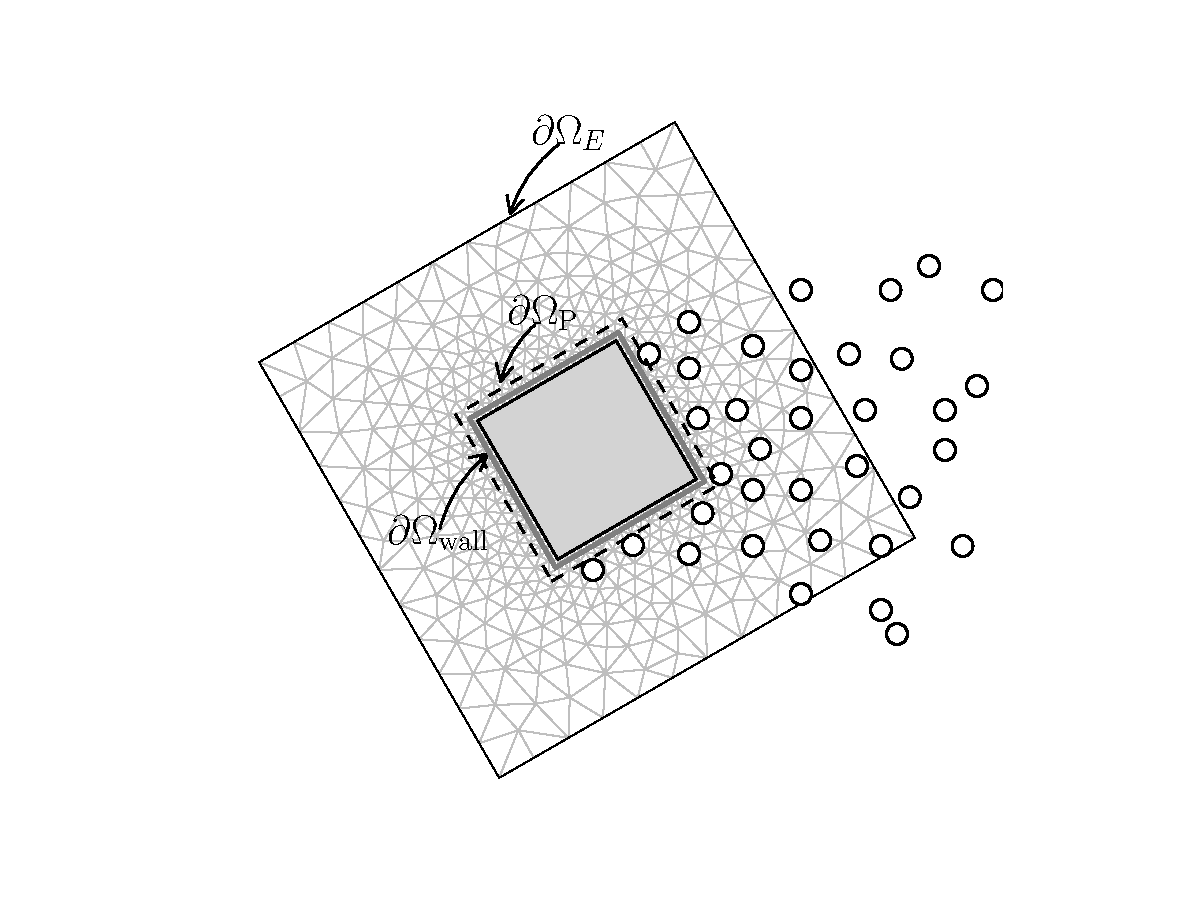
\includegraphics[trim=3.9cm 1.6cm 3.3cm 1.6cm, clip,  width=0.5\linewidth]{./figures/hybrid/interpolation/hybrid.pdf}
	\caption{Boundaries of the hybrid domain}
	\label{fig:hybrid_config}
	\end{figure}	
	%trim=4.37cm 1.58cm 3.86cm 1.58cm, clip,

The coupling of the Eulerian solver and the Lagrangian solver is performed by coupling the solutions of the overlap region $\Omega_E \cap \Omega_L$ according to the procedure of Stock and the Daeninck.

\section{Correction of Lagrangian domain}

The first step of the hybrid coupling scheme is to transfer the highly resolved Eulerian solution to the Lagrangian domain. This is performed by transferring the vorticity in the Eulerian domain $\Omega_E$ onto the vortex blobs that are inside the Eulerian region, $\mathcal{P}: \mathcal{P} \in \Omega_E \cap \Omega_B$.
				
\subsection*{Approach from literature}		
							
However, as Stock has described \cite{} and shown by Daeninck in figure \ref{fig:daeninck_CylinderVorticity}, the Eulerain solution is assumed to be correct from the body up to ``somewhat inside of the outer Eulerian domain", and the Lagrangian solution is valid outside of the outer Eulerian boundary. 

	\begin{figure}[h]
	\centering
	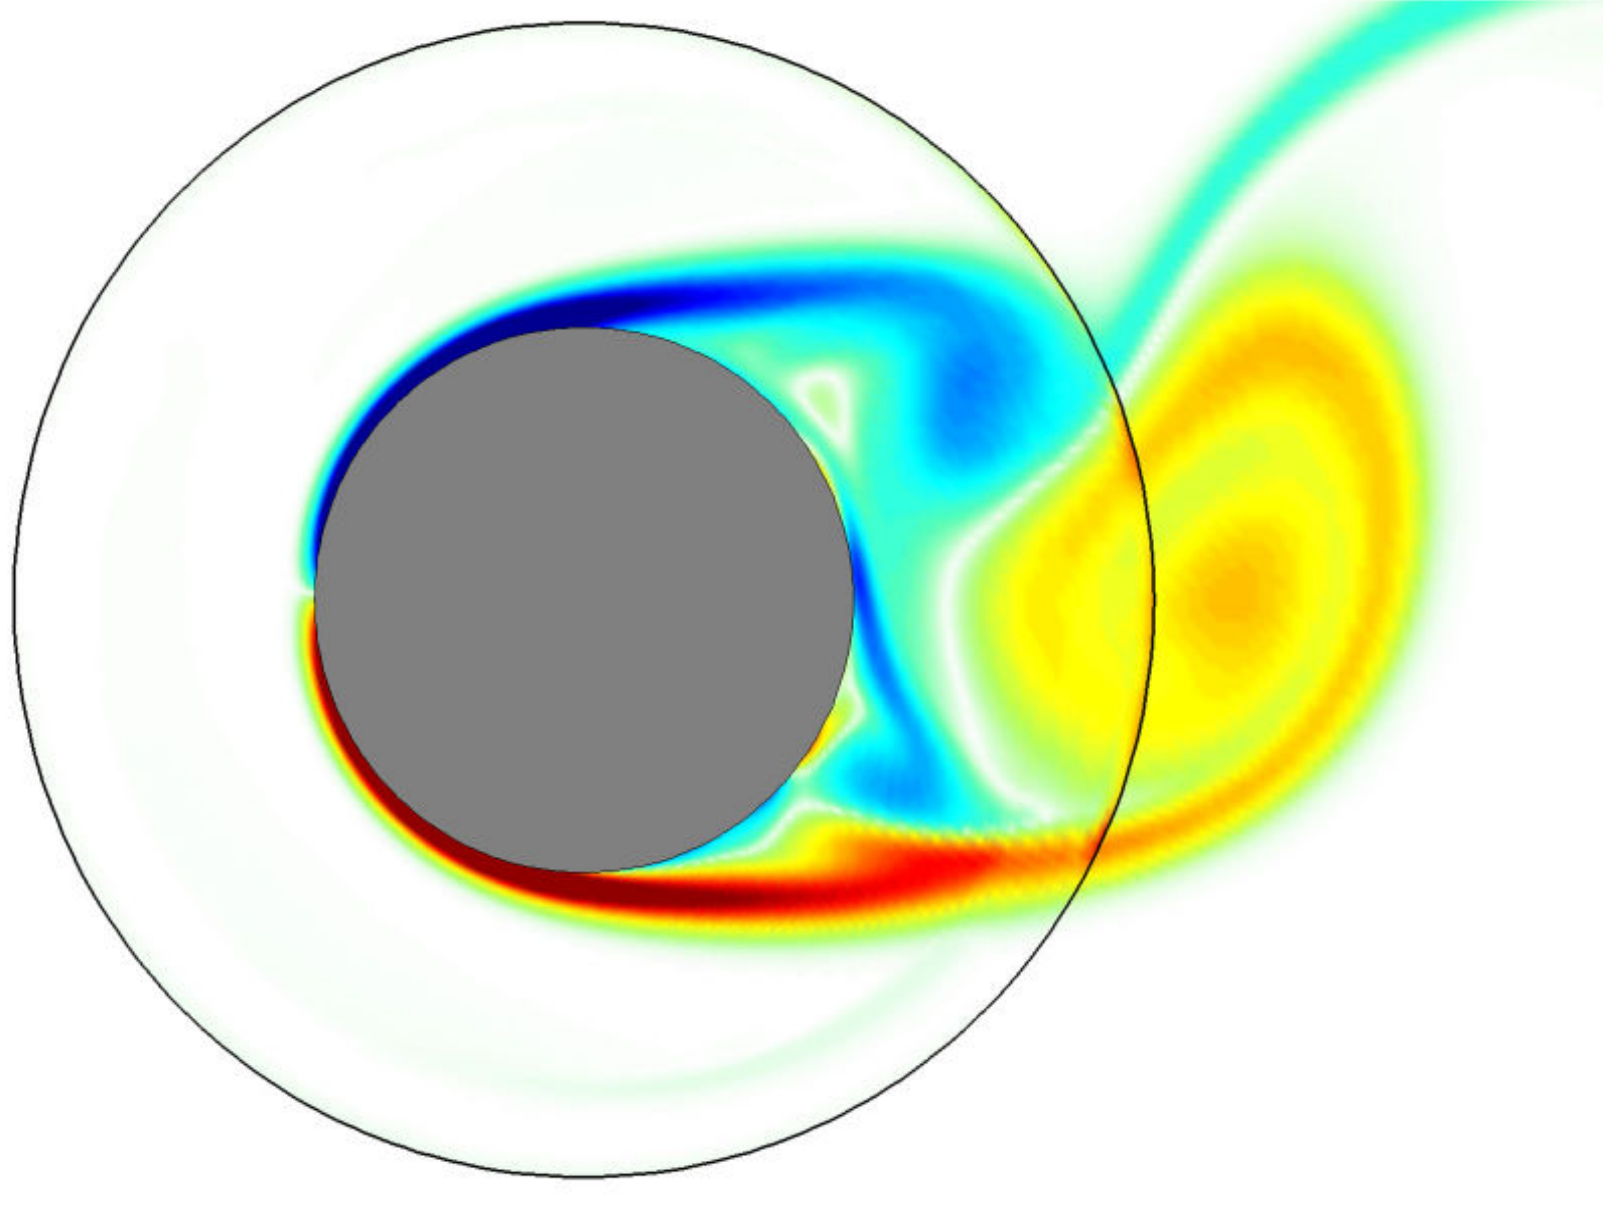
\includegraphics[width=0.5\linewidth]{./figures/hybrid/daeninck_CylinderVorticity.png}
	\caption{Daeninck artificial vorticity at the boundary}
	\label{fig:daeninck_CylinderVorticity}
	\end{figure}

At the boundary of the Eulerian boundary $\partial \Omega_E$, the figure \ref{}, shows artificial vorticity due to slight difference in the solution. To overcome this problem, Stock proposed to interpolate only part of the Eulerian domain onto the Lagrangian domain, as shown in figure \ref{fig:interpRegion}. The interpolation region $\Omega_{int}$ ignores the boundary layer region with the very strong vorticity gradients (which will be resolved by the vortex panel), and part of the outer Eulerian boundary where the Eulerian solution is less accurate. So the interpolation region has the following properties:

	\begin{itemize}
	\item The domain is within the overlap region, $\Omega_{int} \subseteq \Omega_E \cap \Omega_B$,
	\item The domain is bounded by the boundary $\partial \Omega_P$ near the wall with an offset of $d_{surf}\cdot h$ from the surface $\partial \Omega_{\mathrm{wall}}$.
	\item The domain is bounded by the boundary $\partial \Omega_{int}$ at the outer boundary with an offset of $d_{bdry}\cdot h$ from the outer Eulerian boundary $\partial \Omega_{E}$.
	\end{itemize}

	\begin{figure}[t]
     \centering
     \begin{subfigure}[t]{0.35\textwidth}
             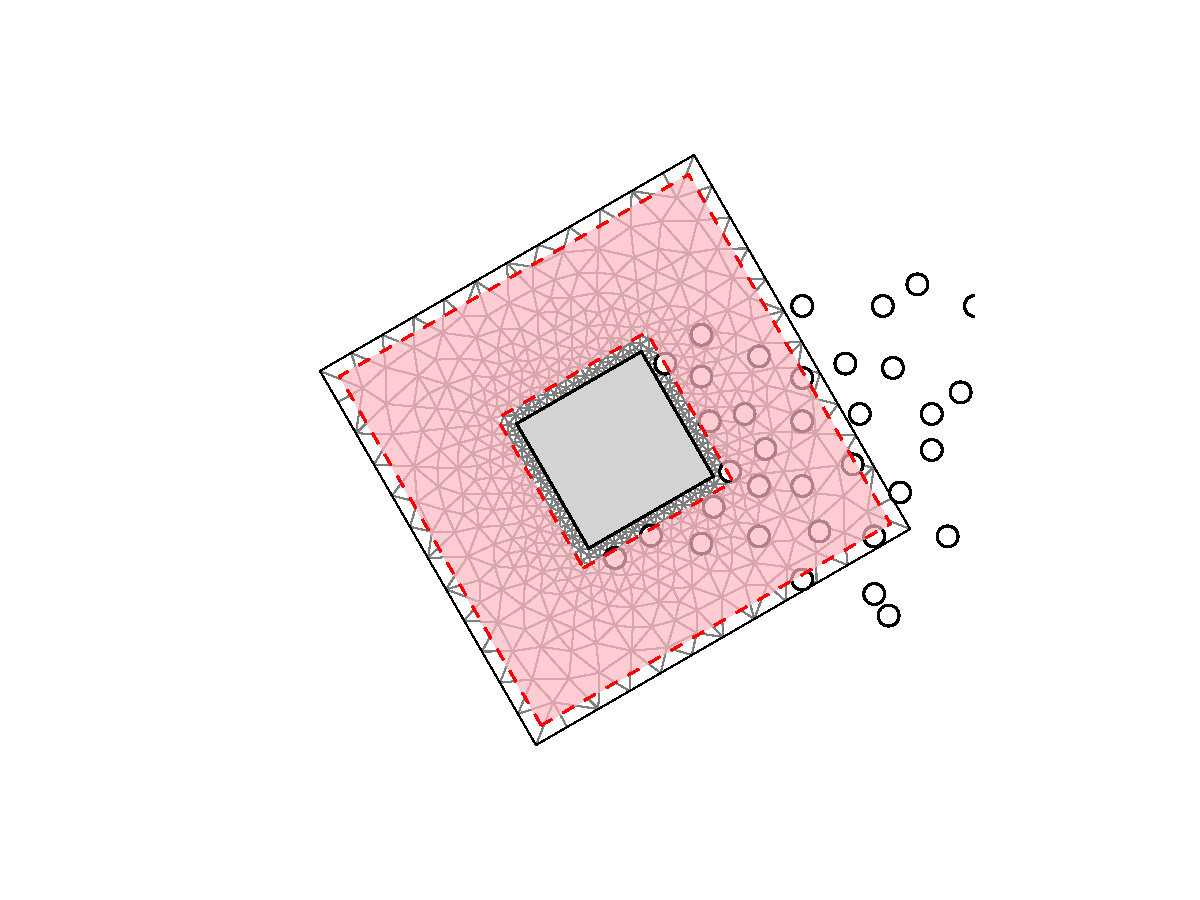
\includegraphics[trim=4.37cm 1.58cm 3.86cm 1.58cm, clip, width=\linewidth]{./figures/hybrid/interpolation/interpRegion.pdf}
             \caption{interpolation region}
             \label{fig:interpRegion}
     \end{subfigure}%
     ~ %add desired spacing between images, e. g. ~, \quad, \qquad etc.
       %(or a blank line to force the subfigure onto a new line)
     \begin{subfigure}[t]{0.6\textwidth}
             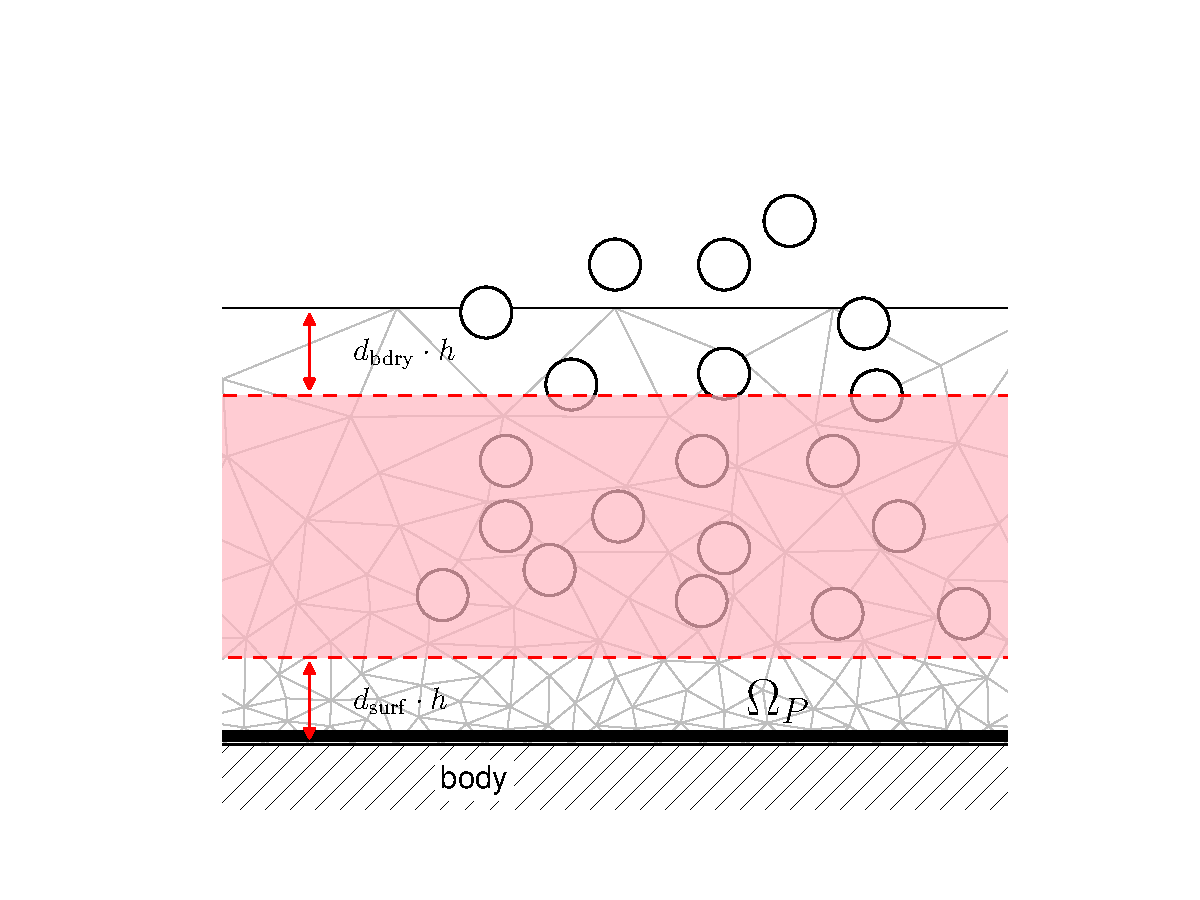
\includegraphics[width=\linewidth]{./figures/hybrid/interpolation/hybrid_domains_withInterpReg.pdf}
             \caption{Interpolation regions}
             \label{fig:hybrid_domains_withInterpReg}
     \end{subfigure}

     \caption{Interp regigs}
     \label{fig:interpolationRegionDefinitions}
	\end{figure}	

The summary of the interpolation algorithm for transferring the Eulerian solution to the vortex blobs used by Stock based on work of Daeninck and Guermond \& Lu is as follows:
\begin{enumerate}
\item Interpolate the solution from Eulerian domain onto a temporary structured grid. Ignore very strong vorticity at the boundary layer, $\mathbf{x} \in \Omega_P$.
\item Determine the locations of the particles inside the interpolation region $\Omega_{int}$. Fill gaps in the region with zero-strength particles. 
\item Reset the strengths of the particles $\mathbf{x}_i$ inside the interpolation region $\Omega_{int}$, figure \ref{fig:interpRegion}, using the local particle volume and the vorticity interpolated from the grid (i.e $\alpha_i = \omega_i\cdot{h^2}$).
\end{enumerate}

Though, through our research we have determined that this approach suffers from issues and does not guarantee the conservation of circulation. 

\subsection*{Issues with the coupling algorithm}

The two main issues with the above approach is as follows:

\begin{itemize}
\item The vorticity bounded to the solid wall was not interpolated to the vortex blobs. 
\item The second issue is that the particle strengths are initialized using standard cell circulation equation, $\alpha_i = \omega \cdot h^2$. This is the standard approach used by the vortex particle community however, this method does not ensure accurate interpolation of the vorticity field, as described by Barba \& Rossi \cite{Barba2010a}.
\end{itemize}

\subsubsection*{Vorticity at the solid wall}

%Therefore to overcome this issue we propose to prescribe the total circulation of the panels such that the circulation is conserved globally.

%\subsubsection*{Prescribed panel strengths}


The first problem that we are concerned is that the vorticity bounded at the solid wall was not transfered to the Lagrangian domain. This is especially problematic in our case as the vortex panel that we have implemented does not diffuse their strength to the vortex blobs. We have implemented the approach used by Daeninck, where the vorticity generated at the wall boundary is introduced from the Eulerian domain. 

To ensure that circulation is conserved, the circulation in the vortex panel domain $\Omega_P$ must be somehow introduced to the Lagrangian domain. Furthermore, if the geometry is at motion, the body itself will have circulation due to the rotation, given as:
	\begin{equation}
	\Gamma_{\mathrm{body}} = \iint\limits_{\mathrm{body}} \nabla \times \mathbf{u}_b \ d A.
	\end{equation}

Therefore, in order to ensure conservation of the circulation, we proposed to transfer the circulation of the domain $\Omega_P$ and the circulation inside the body $\Omega_{\mathrm{body}}$ to the panels.


\subsubsection*{Vorticity Field interpolation error}
	
The second issue we must tackle is the interpolation error that arises due to the standard approach of initializing the particles using the local particle volume and the local vorticity,
	\begin{equation}
	\alpha_i = \omega_i\cdot{h^2},
	\end{equation}
where $i$ corresponds to the vortex blobs $\mathbf{x}_i \in \Omega_{int}$. We summarized this issue in the section \ref{} of the Lagrangian chapter and was extensively investigated by Barba \& Rossi \cite{Barba2010a}. To solve the wake domain of the fluid, we used a vortex particle method that discretizes the vorticity field using $N$ quadrature points,
\begin{equation}
\omega \approx \omega^h(\mathbf{x}_j) = \sum_{i=1}^N \alpha_i \delta(\mathbf{x}_j - \mathbf{x_i}).
\end{equation}

We smoothed the singular kernel $\delta$ by using a Gaussian kernel $\zeta_{\sigma}$. This approach of using vortex blobs is common in the field of vortex particle method and ensures smooth vorticity field. However, the downside to this approach is that on top of the discretization error, we know introduce a so called ``smoothing error" or the ``regularization error" due to the use of gaussian kernel. This is equivalent to blurring the vorticity field, as explained by Barba \& Rossi \cite{Barba2010a}, and the cumulative error in the initialization error is given as

\begin{equation*}
\mathrm{Initialization\ Error} = \mathrm{Smoothing\  Error} + \mathrm{Discretization\ Error}
\end{equation*}

To perform accurate interpolation of the vorticity $\omega$ inside the interpolation domain $\Omega_{int}$ onto the particles $\mathbf{x}_j \in \Omega_{int}$, we must satisfy the following interpolation problem:
	\begin{equation}
	\omega(\mathbf{x}_j) = \hat{\omega}(\mathbf{x}_j),
	\end{equation}
where
	\begin{equation}
	\hat{\omega}(\mathbf{x}) = \sum_{i=1}^{N} \alpha_i \zeta_{\sigma}(\mathbf{x}_j - \mathbf{x}_i),
	\end{equation}
is the discrete vorticity field represented by the linear combinations of the gaussian basis function $\zeta_{\sigma}$ with the vortex blob strength $\alpha_i$. Therefore, assuming the $\alpha_i = \omega(\mathbf{x}_i)\cdot{h^2}$ is incorrect.

As discussed in the secion \ref{} of the Lagrangian chapter, one would assume that the strengths of the particles can be determined by solving the following linear system of equations:
\begin{equation}
\mathbf{A}_{ij}\alpha_i = \omega_i,
\end{equation}
where 
\begin{equation}
\mathbf{A}_{ij} = \zeta_{\sigma}(\mathbf{x}_j-\mathbf{x}_i).
\label{eq:initialization}
\end{equation}

However inverting the matrix $\mathbf{A}$ is still an open question, as stated by Koumoutsakos \& Cottet \cite{}. The problem is that the matrix $\mathbf{A}$ is full and badly condition for direct inversion. For a global field interpolation (i.e for unbounded domain), one could use the Beale's iterative method which uses a \printAcron{successive over-relaxation}{SOR} for solving the equation \ref{eq:initialization}. This method relies on iterative correction of all the particles $\mathbf{x}_i \in \Omega_L$, the Lagrangian domain. 

In our case of initializing the strengths of the particles $\mathbf{x}_i$ in the sub-domain $\Omega_{int}$, it would require us to modify the strength of all the particles $\mathbf{x}_i$ in all $\Omega_B$. This is not feasible not feasible as the size of the problem is very large when the wake is fully developed ($10^5 \leqslant N_{\mathrm{blobs}}$).

Therefore, currently the best possible way of ensure minimal interpolation error from Eulerian domain onto vortex blobs is to perform the following steps:
\begin{itemize}
\item Minimize the smoothing and discretization error by maximizing the particle resolution, achieved by setting $Ov=1$ and reducing $\sigma$ such that the relative error $\epsilon \leqslant 5\%$.
\item As conservation of circulation is a key requirement in fluid dynamic simulation, we ensure that conservation of circulation is not violated when initializing the particles inside the domain $\Omega_{int}$.
\end{itemize}


\subsection{Modified coupling strategy}

The modified version of the hybrid coupling algorithm into five sub-steps
\begin{enumerate}
\item \textbf{Probe vorticity}: Interpolate the vorticity from the Eulerian finite element space onto a uniform structured grid.
\item \textbf{Remove particles}: Remove particles that are inside the interpolation domain $\Omega_{int}$.
\item \textbf{Generate particles}: Generate zero-strength particle inside 
\item \textbf{Assign strengths}: Using the local volume and sldada.. assign the strength of the particles
\item \textbf{Conserve circulation}: Determine the mismatch in the total circulation of the Lagrangian field as determine the strength of the panels such that circulation is conserved.
\end{enumerate}

\subsubsection*{Probe vorticity}

The first step of the hybrid coupling algorithm is to interpolate the vorticity $\omega$ from the the scalar-value function space $W$ onto a structured grid $\hat{\mathbf{x}}$ that follows and covers the entire Eulerian grid.



The vorticity of the Finite element space is probed.

\subsubsection*{Remove particles}

Remove particles inside the interpolation domain.

\subsubsection*{Generate particles}

\subsubsection*{Conserve circulation}

Solve for panel strengths
% of the Eulerian domain overlapping with the vortex panel domain $\Gamma_P \in \Omega_E \cap \Omega_P$ should be transfered to the vortex panels of the Lagrangian domain. In the section \ref{} of the Lagrangian chapter, we have determined that in the case of rotating body, we have to take in account of the circulation inside the body,
%
%Therefore, the total circulation assigned to the vortex panel must be:
%\begin{equation}
%\Gamma_{\gamma} = \oint \gamma(s) \ \mathrm{d}s = \Gamma_P + \Gamma_{\mathrm{body}}
%\label{eq:panelCirculationAreaIntegral}
%\end{equation}
%
%where $\Gamma_P$ is the circulation of the wall region ignored in the Eulerian domain,
%\begin{equation}
%\Gamma_P = \iint\limits_{\Omega_P} \omega \ \mathrm{d}A.
%\end{equation} 
%
%Equation \ref{eq:panelCirculationAreaIntegral} can be simplified using the Stokes' theorem,
%\begin{equation}
%\Gamma_{\gamma} = \oint\limits_{\partial \Omega_P} \mathbf{u}\cdot\mathrm{d}\mathbf{s}.
%\end{equation}

%\subsubsection*{Modified particle correction}
%
%The second problem that we are concerned with is the initialization method to assign the strengths of the particles inside the interpolation region, $\mathbf{x} \in \Omega_{int}$. 
%
%We discussed the problem of initializing the strengths of the blobs $\alpha_i$ as
%\begin{equation}
%\alpha_i = \omega_i \cdot h^2
%\end{equation}
%in section \ref{} of the Lagrangian chapter. This is a common assumption used in the field of vortex particle method for initializing the strengths of the particles in the Lagrangian domain. 
%
%%Therefore, by using Stokes' formulation, we can transfer the ignored circulation of the domain $\Omega_P$ and furthermore, the circulation inside a rotating body.



% Basic approach
% Correction region
%\subsection*{Correction region}


% Problem with the standard approach
% Definition of the interpolation region
% Error in conservation of the circulation


%\subsection{Interpolate Vorticity to Structured grid}
%
%\subsection{Determine blob position and strength}
%
%\subsubsection*{title}


% - Coupling strategy.
% - Features
%%\subsection{Assumptions and Limitations}


%\subsection{Correction of the Lagrangian domain}
% - Stocks modifications

\section{Evolution of the Lagrangian domain}
% - Advance lagrangian solution, Chapter lagrangian explains the algorithm

\section{Evolution of the Eulerian domain}
% - Boundary conditions, all dirichlet from lagrangian

\subsection{Dirichlet boundary conditions}

\subsection{Multi-step evolution}
% Evolution, neglect the pressure b.c, and evolve the problem
% sub

When coupling with the Lagrangian method, we will see that $\Delta t_E \leqslant \Delta t_L$ (Lagrangian time step size is ideally larger than Eulerian time step size), meaning that we will have to perform $k_E$ Eulerian sub-steps to reach the Lagrangian step, figure \ref{fig:multiStep}.

	\begin{figure}[t]
	\centering
	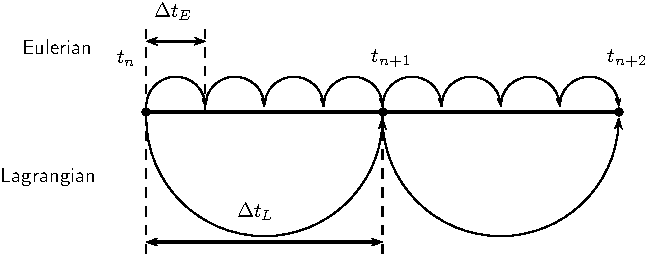
\includegraphics[width=0.7\linewidth]{./figures/eulerian/multiStep-crop.pdf}
	\caption{Eulerian multi-stepping to match the lagrangian $\Delta t_L$. The figures shows $\Delta t_L = 4 \Delta t_E$ and required $k_E = 4$ iterations to time march from $t_n$ to $t_{n+1}$.}
	\label{fig:multiStep}
	\end{figure}	




%	\begin{figure}[t]
%	\centering
%	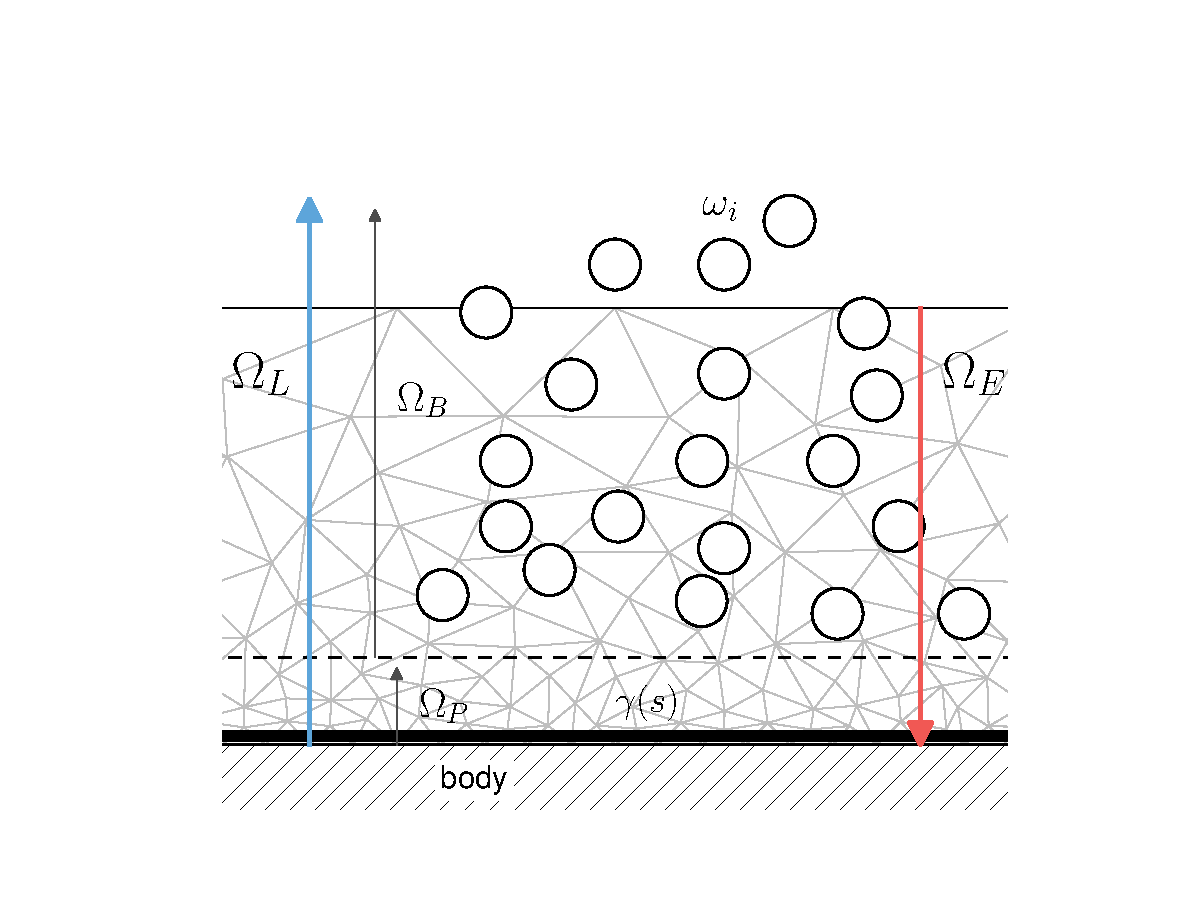
\includegraphics[width=0.7\linewidth]{./figures/hybrid/interpolation/hybrid_domains.pdf}
%	\caption{hybrid domains}
%	\label{fig:hybrid_domains}
%	\end{figure}
%	
%		\begin{figure}[h]
%		\centering
%		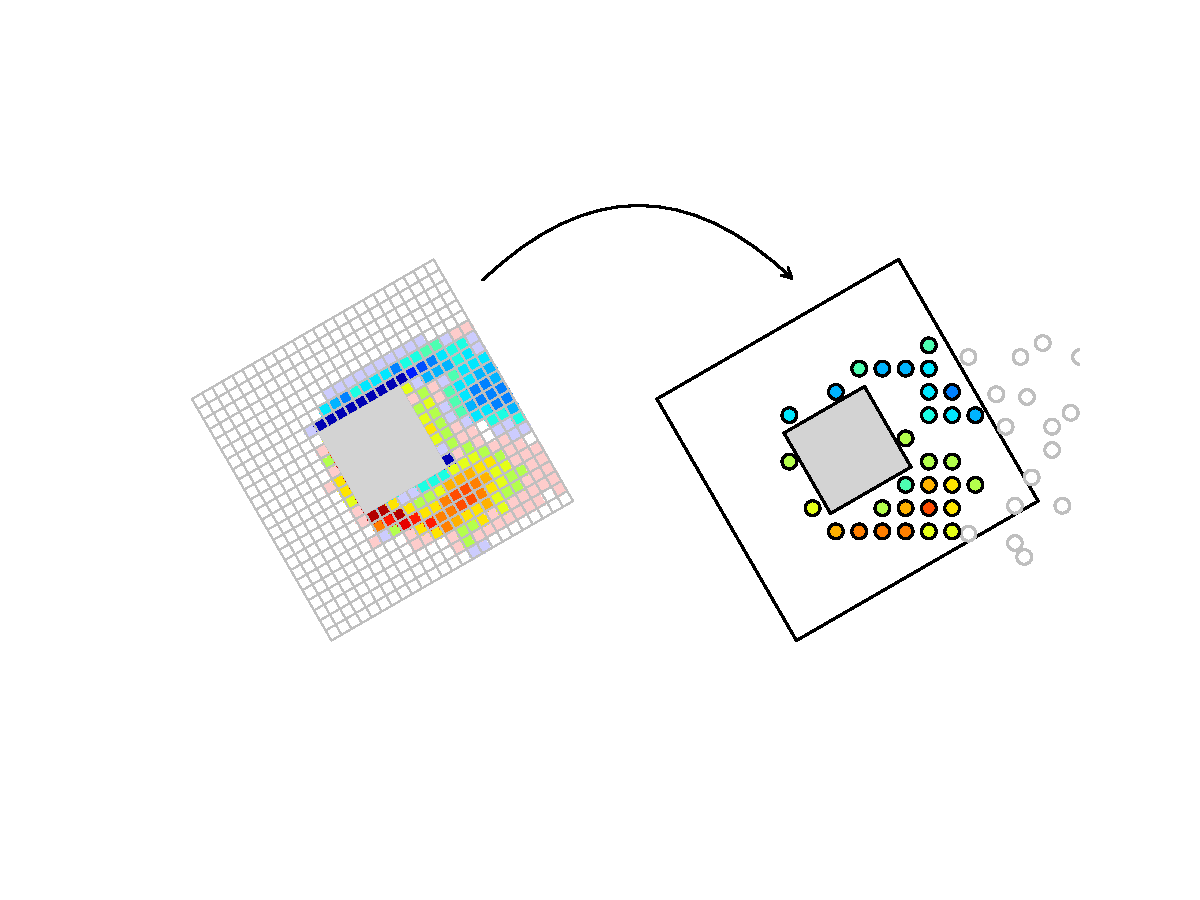
\includegraphics[trim=2.55cm 3.35cm 2.05cm 3.35cm, clip, width=\linewidth]{./figures/hybrid/interpolation/interpolation_StructuredGrid2Blobs.pdf}
%		\caption{interpolation FE2StructuredGrid withData}
%		\label{fig:testFig}
%		\end{figure}




%\subsection{Modified coupling strategy}
%\section{Theory}
%% What is hybrid vortex method?
%% What is the general idea behind the hybrid vortex method?
%% What does it mean to couple particle solver and grid solver?



%	\begin{figure}[h]
%	\centering
%	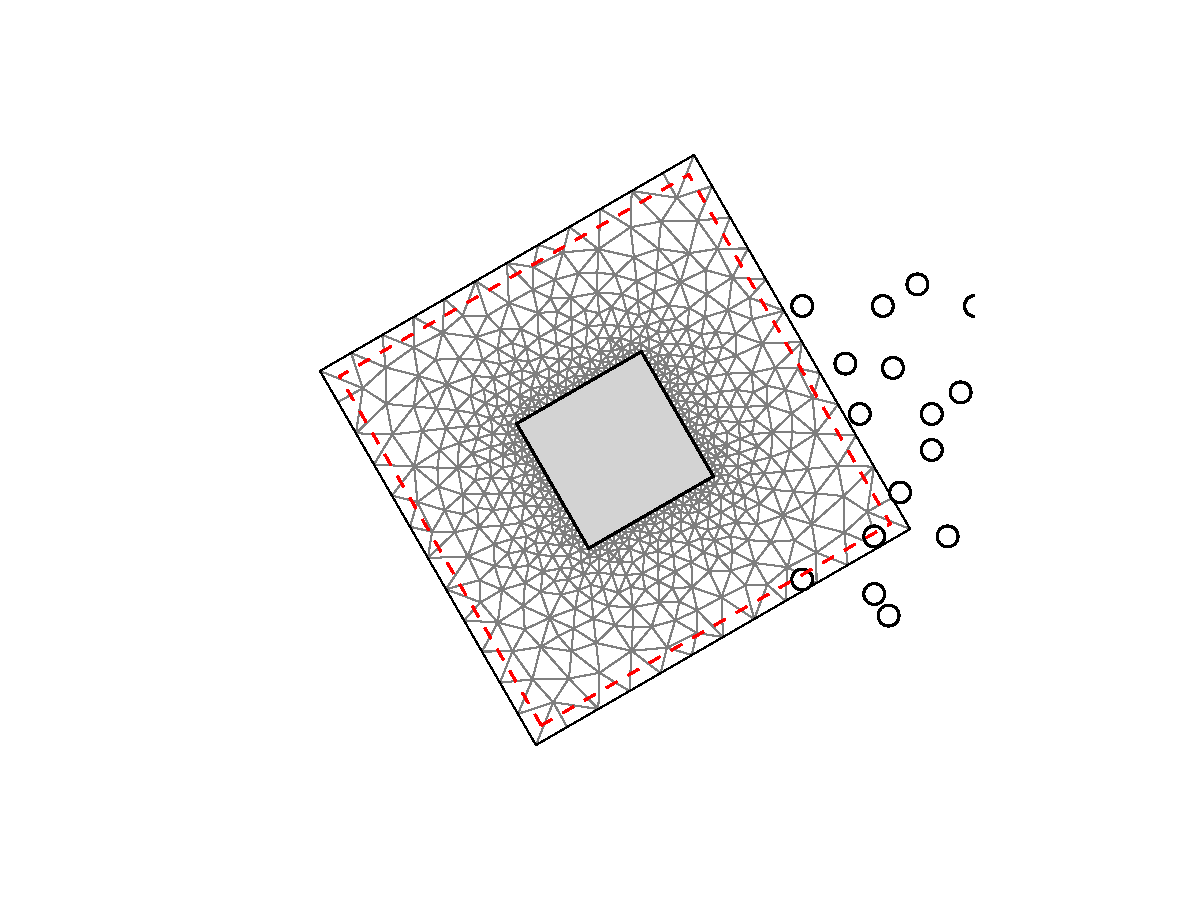
\includegraphics[trim=4.37cm 1.58cm 3.86cm 1.58cm, clip, width=0.5\linewidth]{./figures/hybrid/interpolation/particleRemoved.pdf}
%	\caption{interpolation FE2StructuredGrid withData}
%	\label{fig:testFig}
%	\end{figure}	
	
%	\begin{figure}[h]
%	\centering
%	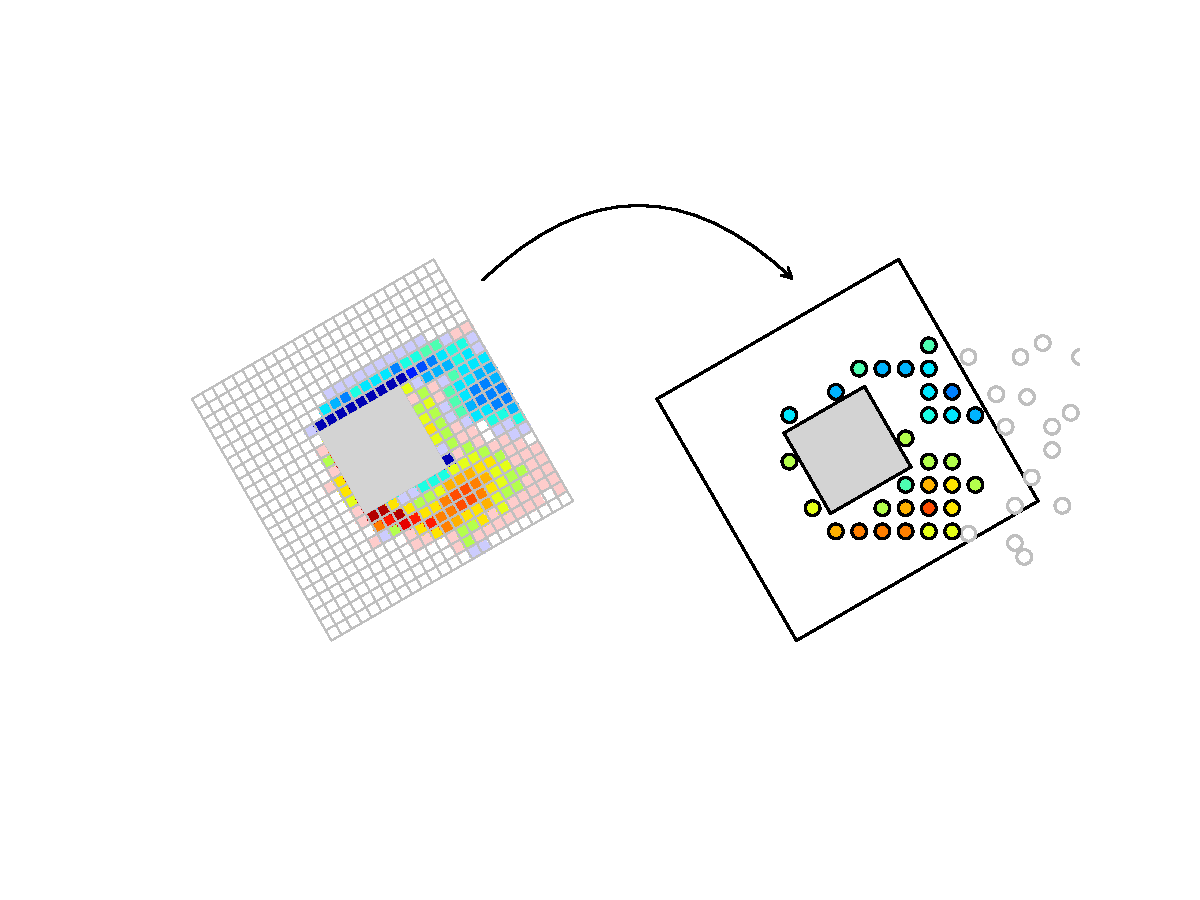
\includegraphics[trim=2.55cm 3.35cm 2.05cm 3.35cm, clip, width=\linewidth]{./figures/hybrid/interpolation/interpolation_StructuredGrid2Blobs.pdf}
%	\caption{interpolation FE2StructuredGrid withData}
%	\label{fig:testFig}
%	\end{figure}		


%\subsection{Eulerian dirichlet boundary condition}
%
%	
%	\begin{figure}[t]
%	\centering
%	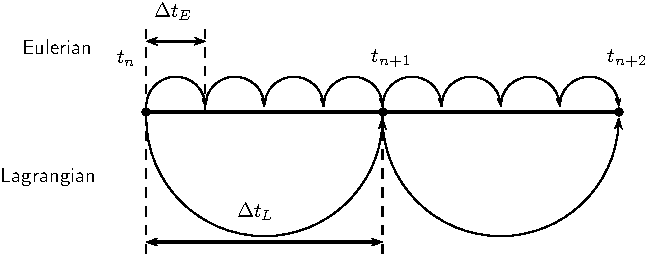
\includegraphics[width=0.7\linewidth]{./figures/eulerian/multiStep-crop.pdf}
%	\caption{Eulerian multi-stepping to match the lagrangian $\Delta t_L$. The figures shows $\Delta t_L = 4 \Delta t_E$ and required $k_E = 4$ iterations to time march from $t_n$ to $t_{n+1}$.}
%	\label{fig:multiStep}
%	\end{figure}	
%
%
%When coupling with the Lagrangian method, we will see that $\Delta t_E \leqslant \Delta t_L$ (Lagrangian time step size is ideally larger than Eulerian time step size), meaning that we will have to perform $k_E$ Eulerian sub-steps to reach the Lagrangian step, figure \ref{fig:multiStep}.

%\subsection{Vorticity interpolation algorithm}

\section{Introduction to pHyFlow: Hybrid solver}
\subsection{Program structure}

\section{Summary}



%
%\section{Particle-Grid Coupling techniques}
%% Multiple ways of coupling , VIC, domain decomposition technique
%\subsection{Vortex in Cell method}
%
%\subsection{Particle-Grid domain decomposition methods}
%
%\section{Vortex diffusion methods}
%
%\subsection{Random walk method}
%\subsection{Core expansion method}
%\subsection{Particle-Strength Exchange}
%\subsection{Modified interpolation kernel for diffusion}
%
%\section{Simulation acceleration techniques}
%
%\subsection{Fast multi-pole Method}
%
%\subsection{Parallel computation in GPU}

%\section{Former Work}
%\label{sec:FormerWork}
%
%\subsection{Overview of the Work}
%\label{subsec:OverviewoftheWork}

%\section{Purpose of further research}

%%%%%%%%%%%%%%%%%%%%%%%%%%%%%%%%%%%%%%%%%%%%%%%%%%%%%%%%%%%%%%%%%%%%
%\nomenclature[ak]{$K$}{Kelvin (temperature)}
%\nomenclature[ar]{rpm}{Revolutions per minute (frequency)}
%\nomenclature[ac]{CO}{Carbon Monoxide}
%\nomenclature[ac]{CRM}{Chemical Reaction Modelling}
%\nomenclature[ah]{H2}{Molecular hydrogen}
%\nomenclature[ag]{GSP}{Gas Turbine Simulation Program (Software)}
%\nomenclature[rr]{$\rho$}{Density \nomunit{[$kg/{m^3}$]}}
%\nomenclature[sm]{$\dot{m}$}{Mass flow rate \nomunit{[$kg/s$]}}
%\nomenclature[ab]{bar}{Pressure}

%\nomenclature[rr]{$Re$}{Reynolds number \nomunit{[-]}}
%\nomenclature[rw]{$M$}{Mach number \nomunit{[-]}}
%\nomenclature[rw]{$\mu$}{Dynamic viscosity of air \nomunit{[$kg/{s \cdot m}$]}}